\documentclass[12pt, a4paper]{article}
\usepackage{amsmath}
\usepackage{graphicx}
\usepackage{tabularx}
\usepackage{enumerate}
\usepackage{enumitem}
\usepackage{chngpage} % temp change margins for large tables
\usepackage[margin=1in]{geometry}
\usepackage[open]{bookmark} %pdf bookmarks
\usepackage{hyperref}
\hypersetup{pdfstartview={XYZ null null 1.00}} % pdf zoom 100%
\usepackage{caption} % these 2 for subfigures
\usepackage{subcaption}
\usepackage{float} % for extra float options such as [H] after \begin{figure}
\usepackage[normalem]{ulem} % for strikethrough \sout{text}
\linespread{1.3}
\usepackage{titlesec}
\setlength{\parindent}{0pt}
\setlength{\parskip}{1em}
\titlespacing*{\section}{0pt}{0cm}{0cm}
\titlespacing*{\subsection}{0pt}{0cm}{-0.2cm}

\begin{document}
%\title{\vspace{-2.0cm}Cascade Experiment}
%\author{\vspace{-5.0cm}CCN: 5726A}
%\date{\vspace{-2.0cm}26/10/2021}
%\maketitle

\begingroup  
\centering
\LARGE 4A2: Computational Fluid Dynamics Final Report\\[1em]
\large CCN: 5726A \\
\large 10/12/2021 \\
\endgroup

%\renewcommand{\thesubsection}5{\arabic{subsection}} % Remove section number from subsection numbering
\section{Summary}
A basic Euler code was developed to solve fluid flows for subsonic and supersonic flows in any geometry. The code was enhanced with 4 extensions: Runge-Kutta, Deferred Correction, Constant Stagnation Enthalpy and Spatially Variable Time Step. The first improved stability, the second improved spatial accuracy and the last two increased speed. Each extension can be turned on or off individually and the overall enhanced code was analysed to see how the maximum CFL, minimum smoothing factor (SF), accuracy, convergence speed and CPU time are affected in comparison to the basic code. Difficulties include the need to alter initial guesses or boundary conditions to guarantee a fully supersonic or subsonic flow for some test cases. Special care had to be taken to choose an appropriate $SF$ low enough to capture shock waves but not too low that the CPU time would be too large, which was difficult at times.

\section{Basic Code and Developments}
\begin{table}[h]
	\centering
	\caption{Basic code performance for test case 0}
	\label{tab:basic}
	\begin{tabular}{|c|c||c|c|c|c|}
		\hline
		& & \multicolumn{4}{c|}{Fastest CPU Time} \\ \hline
		Max. CFL & Min. SF & CFL & SF & Steps & CPU Time (s) \\ \hline
		1.1 & 0.2 & 1.1 & 0.8 & 930 & 0.878 \\ \hline
	\end{tabular}
\end{table}
The basic code was very unstable, inaccurate and slow relative to the enhanced code. As seen in \autoref{tab:basic}, anything beyond $CFL=1.1$ and below $SF=0.2$ made the solution diverge. In the Interim Report, it was found that the basic code took 2000 steps to converge for $CFL=0.5$ and $SF=0.5$. This shows that increasing $CFL$ increases convergence speed by taking larger time steps, and increasing $SF$ also increases convergence speed at the expense of accuracy. At high $SF$ the solution has significant artificial diffusion and the solution led to inaccurate, asymmetric results as seen in \autoref{fig:basic}. Reducing $SF$ improves accuracy but increases convergence speed and loses stability benefits of the smoothing.
\begin{figure}[H]
	\centering
	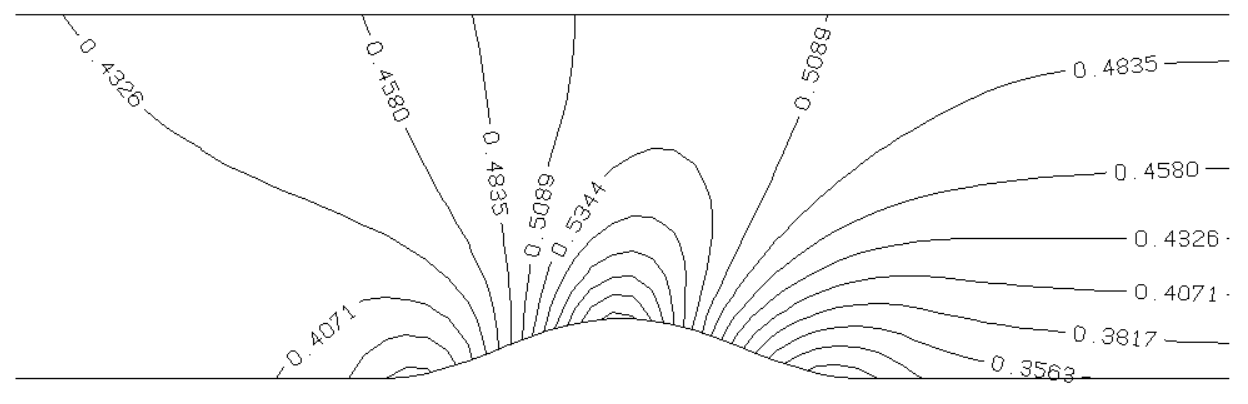
\includegraphics[width=\textwidth]{plots/0 basic best}
	\caption{Mach contour of basic code, test case 0, $CFL=1.1$ $SF=0.8$}
	\label{fig:basic}
\end{figure}

4 Extensions were implemented, each could be enabled or disabled in \textit{Euler.f90}. This allows their effects to be analysed individually, which are shown in \autoref{tab:each}. Other developments include printing to the terminal the average, maximum and minimum outlet Mach numbers. These were used to assess uniformity and the accuracy of the results by comparing to calculated values.

% Table generated by Excel2LaTeX from sheet 'Sheet1'
\begin{table}[htbp]
	\centering
	\caption{Performance of each extension for test case 0}
	\begin{tabular}{|l|c|c||c|c|c|c|c|} \hline
		&       &       & \multicolumn{5}{c|}{Fastest CPU Time} \\ \hline
		& max. CFL & min. SF & CFL   & SF    & Steps & Time(s) & t/Step(s) \\ \hline
		Basic & 1.0     & 0.2   & 1.1   & 0.7   & 920   & 0.945 & 0.001027 \\ \hline
		Runge-Kutta & 5.2   & 0.0007 & 6.0     & 0.15  & 320   & 1.247 & 0.003897 \\ \hline
		Deferred Correction & 0.5   & 0.2   & 0.5   & 0.5   & 2325  & 2.049 & 0.000881 \\ \hline
		Const. $h_0$ & 1.3   & 0.2   & 1.3   & 0.6   & 650   & 0.651 & 0.001002 \\ \hline
		Variable $\Delta t$ & 0.6   & 0.35  & 0.6   & 0.8   & 1115  & 1.098 & 0.000985 \\ \hline
	\end{tabular}%
	\label{tab:each}%
\end{table}%

\subsection{Runge-Kutta}
The Runge-Kutta method improved stability by dividing each time step into 4 sub-steps. The changes in the primary variables calculated in each sub-step were added onto the values of the primary variables at the start of the overall step and the new values were used to find the changes in the next sub-step. The time steps used for the 4 sub-steps were 1/4, 1/3, 1/2 and 1.0 of the main time step. This new loop was implemented in the main \textit{Euler.f90} program, with the new time step multiplier implemented in \textit{sum\_fluxes.f90} as a new parameter.

\autoref{tab:each} shows that the maximum $CFL$ has increased massively to 5.2. This increase in time step led to much faster convergence, from 920 to 320 steps. However, due to the extra iterations within each time step, the CPU time per time step increased significantly, just under 4x the basic code's. As a result the overall CPU time increased slightly. On the other hand, the minimum $SF$ has been reduced significantly. This means at a lower $SF$ the solution was more accurate and gave low numerical results. In other words, the solution is now much more stable. However, a lower $SF$ again leads to a slower convergence.

\subsection{Deferred Correction}
As seen in \autoref{fig:basic}, the significant smoothing, or artificial viscosity caused it to become unsymmetrical and smeared. Deferred correction improved the accuracy by cancelling out most of this artificial artificial without losing the stability benefits. If a correction factor is added on very gradually so that on every time step only a small part of the new correction and a large part of the old one are taken, the stability is maintained while the effective smoothing is reduced significantly.
The proportion of the artificial viscosity that is cancelled was set to $fcorr=0.9$ and this was applied in \textit{smooth.f90} to update the stored correction passed as an argument in this subroutine.

\autoref{fig:0.1mach} shows a very symmetric contour, evidence that the artificial viscosity has been reduced significantly, this means that a higher value of SF could be used to have rapid convergence while maintaining high levels of numerical accuracy. \autoref{tab:each} shows however the maximum $CFL$ has decreased to 0.5, leading to a slower convergence and CPU time. This is acceptable, as the purpose of this method is to improve accuracy.

\subsection{Constant Stagnation Enthalpy}
This simplification was feasible as a result of discarding time accuracy, since we are only interested in the steady solution. The flow is adiabatic and the inlet stagnation enthalpy is fixed, from the steady flow energy equation the stagnation enthalpy must then be uniform throughout the flow. This was set as $h_0=c_p\times T_{0,in}$ in \textit{set\_others.f90} and \textit{apply\_bconds.f90}. "roe" was discarded everywhere including in the main program iteration, this means the pressure was calculated as $p=\rho R T$.

By removing "roe", 1 of 4 primary variables, calculations roughly $25\%$ of the main calculations have been reduced. \autoref{tab:each} shows that the maximum $CFL$ increased to $1.3$, leading to faster convergence and CPU time, with the CPU time per step also decreasing slightly.

\subsection{Spatially Variable Time Step}
Similarly, if time accuracy is discarded, different cells can use different time steps in the solution. This is because the steady state equations reduce to: $\sum (Fluxes\,\Delta t/\Delta vol)=0$. This is satisfied no matter what time step is used. Hence, the time step of each cell now depends on its \underline{local} speed of sound, velocity, and shortest edge: $\Delta t=dmin_{loc}/(c_{loc}+v_{loc})$. These values were taken as averages from the 4 corners of the cell and were updated every 5 steps in the main iteration. 

\autoref{tab:each} shows that the maximum $ CFL $ has now been reduced to $ 0.6 $. This is because the most unstable element was being updated by much less than its stable time step in the basic code but it will now be updated by its own maximum stable time step. Moreover, the minimum $SF$ has increased to $0.35$. As a result convergence and CPU were slower. However, the overall CPU time per step has reduced to $0.000985s$ because the average time step $\Delta t$ has increased. This method is most advantageous when the grid size is not uniform. For our test cases the grids were relatively uniform and the benefits only just outweighed the extra complexity in updating time step sizes.

\section{Test Cases}
Each test case was solved by the enhanced code, which included all 4 extensions described in the previous section. For each case, the maximum $CFL$ and minimum $SF$ were identified. The $CFL$ and $SF$ which led to the fastest convergence speed were found, including the CPU time and CPU time per step. The average outlet Mach number ($M_{out, Avg}$) was found by averaging all Mach numbers at the exit plane. The maximum and minimum outlet Mach were also printed to check how uniform the outlet flow was (for test case 5). These are compared with the expected Mach number ($M_{out, Expected}$), which for test cases 0-3 were calculated using the isentropic relation:
\begin{equation*}
	\dfrac{p_{out}}{p_{0,\,in}} = \left( 1+\dfrac{2}{\gamma-1}M_{out, Expected}^2 \right) ^{\mbox{\footnotesize $-$\large $\frac{\gamma}{\gamma-1}$}}
\end{equation*}

Where $p_{out}$ and $p_{0,\,in}$ are the variables \textit{pdown} and \textit{pstagin} in the code respectively. 

Test case 4's expected exit Mach was calculated using the oblique shock tables for a flow turning of $5.727\,^{\circ}$, which occurred twice (1 reflection). Lastly, test case 5 was designed to accelerate the flow to $M=3$ so that was the Mach expected.

\begin{table}[H]
	\captionsetup{justification=raggedright}
	\begin{adjustwidth}{-0.5in}{-0.5in}
	\centering
	\captionsetup[table]{justification=raggedright}
	\caption{Performance of enhanced code for all cases}
	\begin{tabular}{|l|c|c||c|c|c|c|c|c|c|} \hline
		&       &       & \multicolumn{7}{c|}{Fastest CPU Time} \\  \hline
		Case  & max CFL & min SF & CFL   & SF    & Steps & Time(s) & t/Step(s) & $M_{out,\, Avg}$ & $M_{out,\,Expected}$ \\ \hline
		0     & 3.7   & 0.0013 & 3.7   & 0.25  & 255   & 0.932 & 0.00365 & 0.485 & 0.487 \\ \hline
		1     & 6.3   & 0.007 & 6.3   & 0.15  & 190   & 1.578 & 0.00831 & 1.046 & 1.046 \\ \hline
		2, $85kPa$ & 4.0     & 0.04  & 4.0     & 0.23  & 925   & 5.744 & 0.00621 & 0.486 & 0.487 \\ \hline
		2, $80kPa$ & 4.9   & 0.12  & 2.4   & 0.4   & 995   & 7.166 & 0.00720 & 0.566 & 0.574 \\ \hline
		2, $27kPa$ & 4.5   & 0.09  & 4.5   & 0.09  & 1275  & 7.666 & 0.00601 & 1.451 & \sout{1.501} \\ \hline
		3     & 7.5   & 0.04  & 3.0     & 0.05  & 3625  & 75    & 0.0207 & 1.488 & \sout{1.501} \\ \hline
		4     & 5.3   & 0.04  & 5.3   & 0.1   & 510   & 4.987 & 0.00978 & 1.186 & 1.189 \\ \hline
		5     & 4.7   & 0.08  & 4.7   & 0.2   & 535   & 6.029 & 0.0113 & 2.990  & 3.00 \\ \hline
	\end{tabular}%
	\label{tab:enhance}%
	\end{adjustwidth}	
\end{table}%


\subsection{Test Case 0}
This is a simple subsonic flow over a Gaussian bump in the middle. The geometry is symmetrical so the flow should be expected to be symmetrical too. 

\begin{figure}[H]
	\centering
	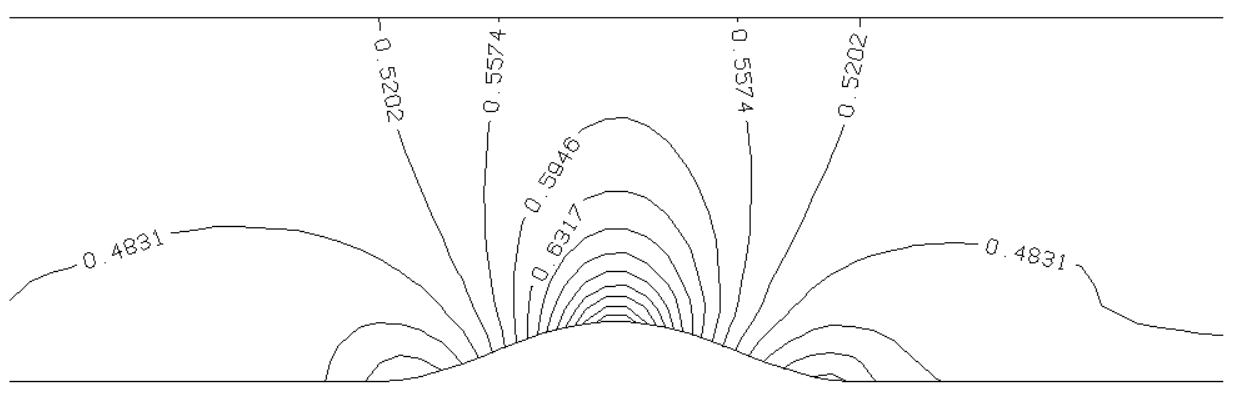
\includegraphics[width=\textwidth]{plots/0.2 mach}
	\caption{Mach contour for best CPU time of test case 0}
	\label{fig:0.2mach}
\end{figure}
\begin{figure}[h]
	\centering
	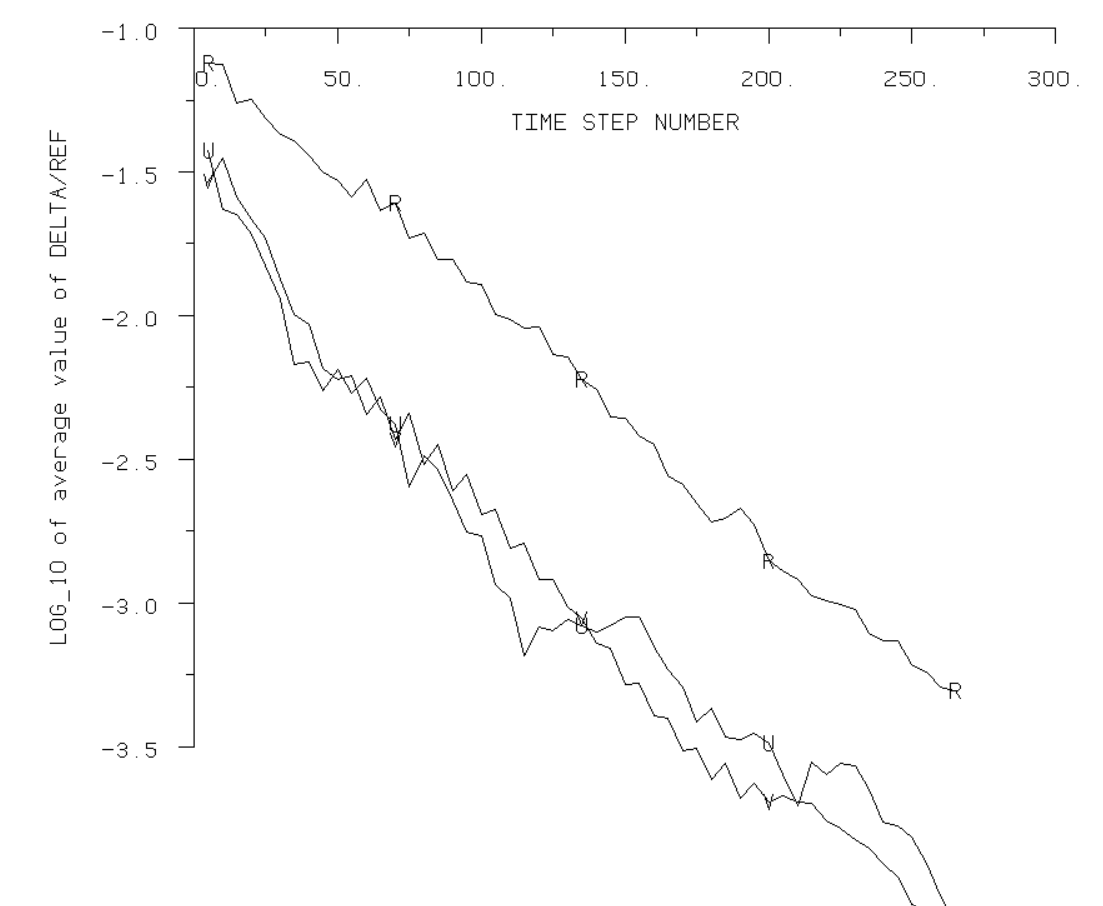
\includegraphics[width=0.7\textwidth]{plots/0.2 conv}
	\caption{Convergence for best CPU time of test case 0}
	\label{fig:0.2conv}
\end{figure}
\begin{figure}[h]
	\centering
	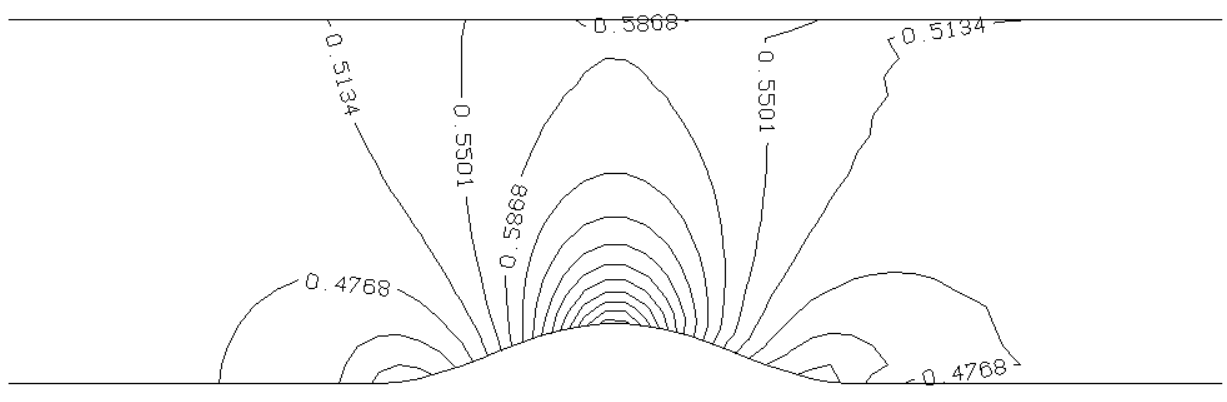
\includegraphics[width=\textwidth]{plots/0.1 mach}
	\caption{Mach contour for minimum $SF$ of test case 0}
	\label{fig:0.1mach}
\end{figure}

Comparing the performance in \autoref{tab:enhance} (Enhanced) and in \autoref{tab:basic} (Basic), it can be seen that the maximum $CFL$ and minimum $SF$ have improved significantly. \autoref{fig:0.1mach} shows that at the minimum $SF$, the lack of smoothing led to the solution being very unstable, with some Mach contour showing discontinuities. A higher $SF$ therefore was chosen for the best result in \autoref{fig:0.2mach}. 

The higher allowed $CFL$ meant the steps to converge reduced greatly from 920 to 255. However, the CPU time per step has increased mainly due to the Rune-Kutta extension. As a result, the overall CPU time remained similar, only reducing by 1.4\%. The minimum $SF$, along with the lower $SF$ for the best CPU time, led to the flow being much more accurate and symmetrical, due to mostly the Deferred Correction extension which removed most of the effective artificial viscosity. This can be seen from \autoref{fig:0.1mach} compared to \autoref{fig:basic}. The outlet Mach number is accurate, only differing to the expected Mach by 0.4\%.

\subsection{Test Case 1}
This is a simple subsonic flow around a 90$^{\circ}$ bend. 
\begin{figure}[H]
	\centering
	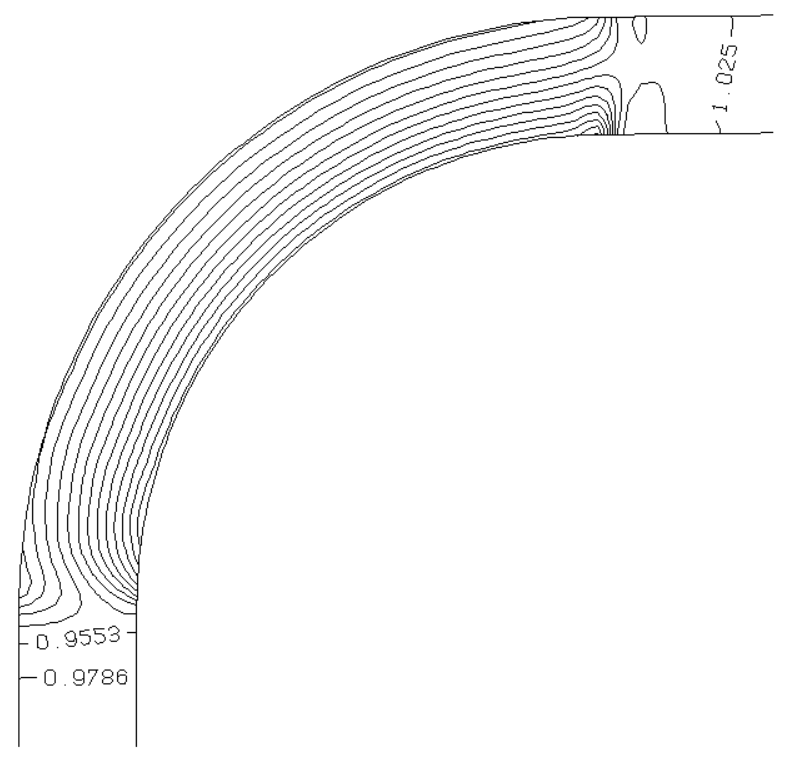
\includegraphics[width=0.7\textwidth]{plots/1.2 mach}
	\caption{Mach contour for best CPU time of test case 1}
	\label{fig:1.2mach}
\end{figure}
\begin{figure}[H]
	\centering
	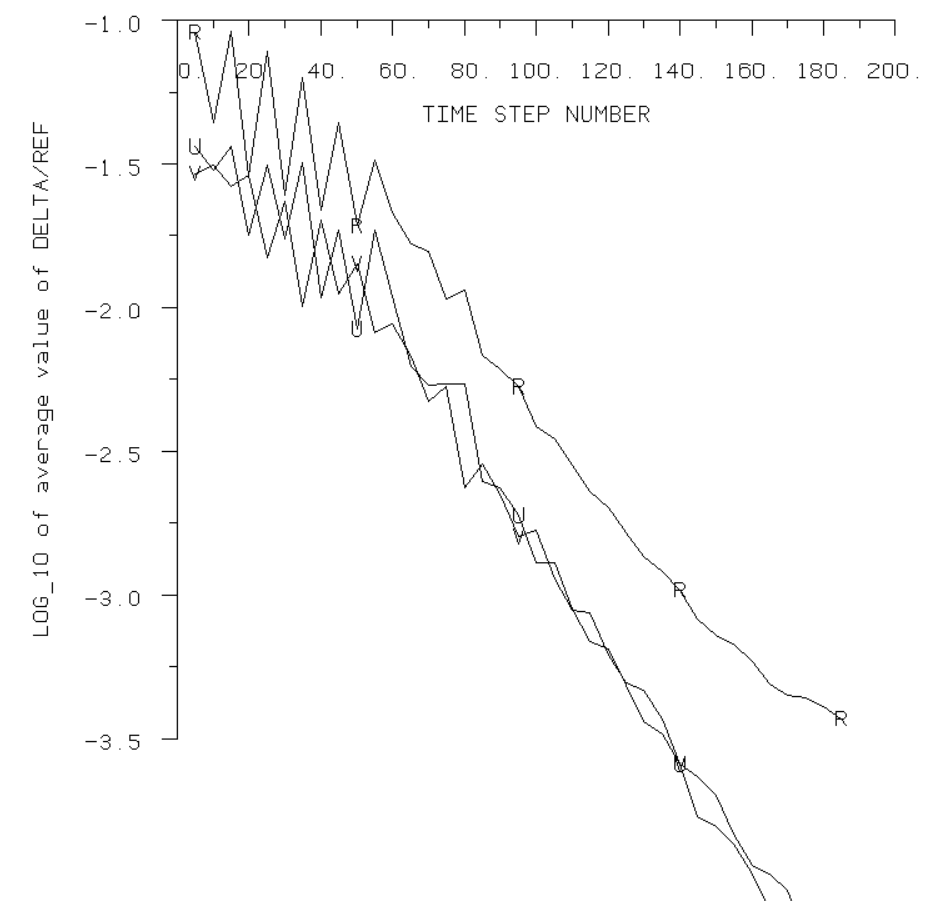
\includegraphics[width=0.7\textwidth]{plots/1.2 conv}
	\caption{Convergence for  best CPU time of test case 1}
	\label{fig:1.2conv}
\end{figure}

The Mach contour in \autoref{fig:1.2mach} shows that the solution is symmetrical about the middle, with the contour lines maintaining the same distance from each other. This demonstrates the lack of artificial diffusion in the solution. The maximum $CFL$ has been increased to an astounding 6.3 (\autoref{tab:enhance}). This led to the steps to converge being at the lowest of the test cases, at 190 steps. Moreover, the measured average outlet Mach equals the expected value, accurate to 3 decimal places, a benefit of the accuracy bonus of Deferred Correction. \autoref{fig:1.2conv} shows the rapid convergence. The residuals fluctuate a lot in the first 60 steps, then become stable and reach convergence quickly.
 
\subsection{Test Case 2}
This is similar to test case 0, a simple bump but with an extended downstream region. This case was run with 3 different back pressures ('\textit{pdown}' in the '\textit{flow}'), 85kPa, 80kPa, and 27.2kPa. 

\begin{figure}[H]
	\centering
	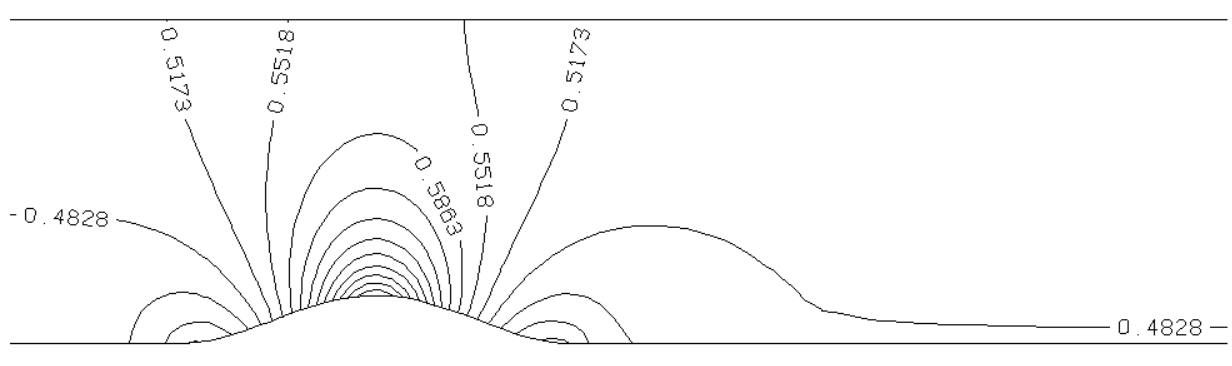
\includegraphics[width=\textwidth]{plots/2.2 mach}
	\caption{Mach contour for best CPU time of test case 2, 85kPa}
	\label{fig:2.2mach}
\end{figure}
Similar to test case 0, \autoref{fig:2.2mach} shows a symmetrical Mach contour, but now also showing how the flow quickly returns to parallel downstream of the bump, which test case 0 did not show. Again the measured outlet Mach is correct to 0.2\%, showing just how accurate this enhanced code is.
\begin{figure}[H]
	\centering
	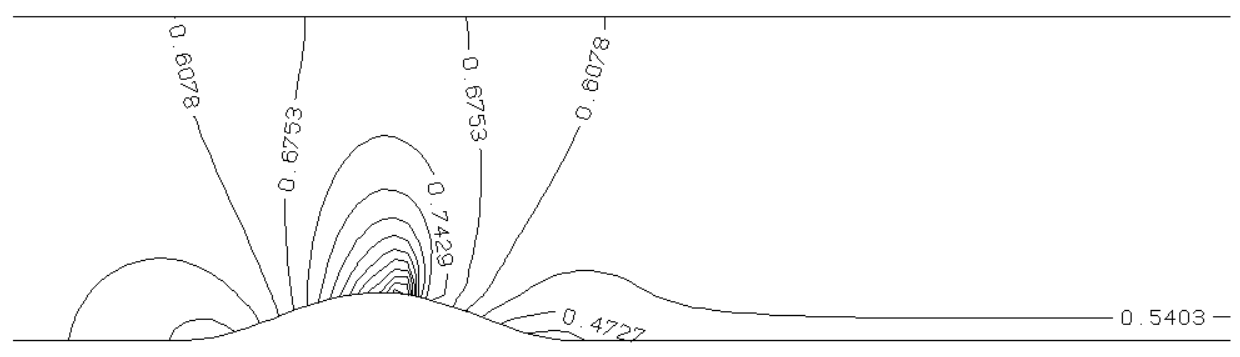
\includegraphics[width=\textwidth]{plots/2.6 mach}
	\caption{Mach contour for best CPU time of test case 2, 80kPa}
	\label{fig:2.6mach}
\end{figure}
With a lower back pressure at 80kPa, the maximum Mach number now exceeds 1, around the throat. This suggests there may be a very weak shock just downstream of the throat which returns the flow back to subsonic. This can be shown in \autoref{fig:2.6mach}, where the contour lines become very dense just aft of the throat. The full shock is not seen because it is a very weak shock, meaning the discontinuity and change in variables are small. The $SF$ chosen was not low enough to capture the full extent of this thin shock, but still low enough to see signs which suggest a shock. This is largely due to Runge-Kutta allowing a much lower $SF$ to be used, while Deferred Correction ensures the solution is accurate.
\begin{figure}[H]
	\centering
	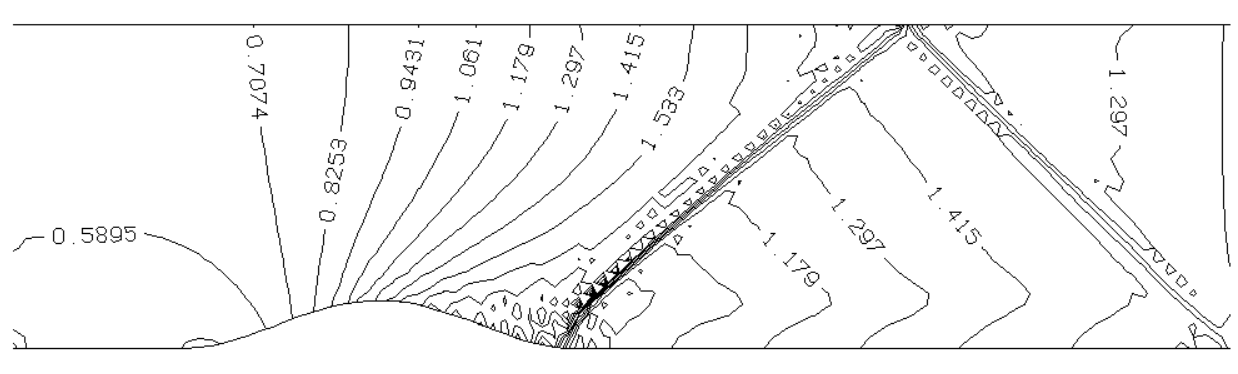
\includegraphics[width=\textwidth]{plots/2.7 mach}
	\caption{Mach contour for best CPU time of test case 2, 27.2kPa}
	\label{fig:2.7mach}
\end{figure}
With an even lower back pressure at 27.2kPa, the bump now acts as an isentropic con-di nozzle, choking at the throat and accelerating the flow to supersonic speeds. However, aft of the divergent section, the supersonic flow is turned to become horizontal again. This flow turning led to the formation of a oblique shock wave which was reflected off the top surface. These 2 oblique shocks decelerated the flow slightly at the outlet. The small enclosed contour lines on either side of the shock are a result of the large discontinuities, leading to relatively unsteady results in these regions. Similarly, at the bottom of the divergent section the flow is unsteady because the flow is turned throughout this whole section, so weaker oblique shocks are formed upstream of the main shock.

These shocks are only captured due to Runge-Kutta allowing a much lower $SF$ to be used, otherwise the shocks would be smoothed out by artificial viscosity. Deferred Correction ensures the shock angle and strength are accurate. As a result of these shocks, the measured outlet Mach cannot be compared to the expected Mach which was calculated assuming shock-free.
\subsection{Test Case 3}
This is a bump as with test cases 0 and 2, but placed in a 180$\,^{\circ}$ bend. The back pressure was 27.2kPa, as with the last run in test case 2, so shocks were expected to be formed downstream of the throat.
\begin{figure}[H]
	\centering
	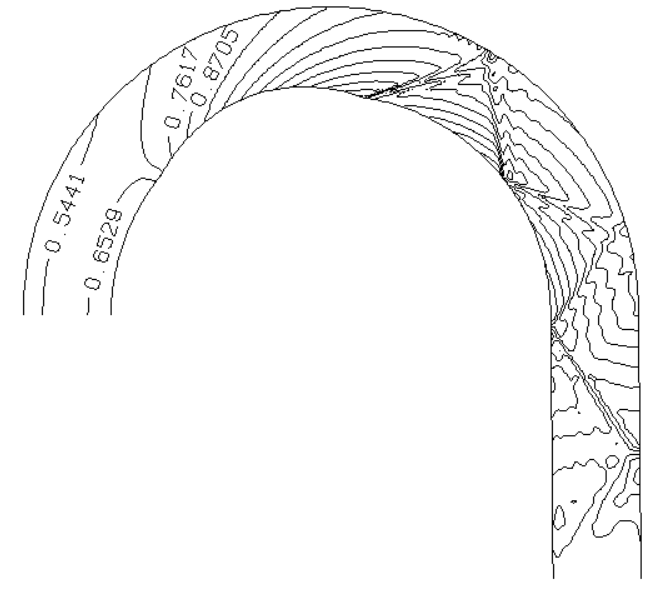
\includegraphics[width=0.7\textwidth]{plots/3.1 mach}
	\caption{Mach contour for  best CPU time of test case 3}
	\label{fig:3.1mach}
\end{figure}
\begin{figure}[H]
	\centering
	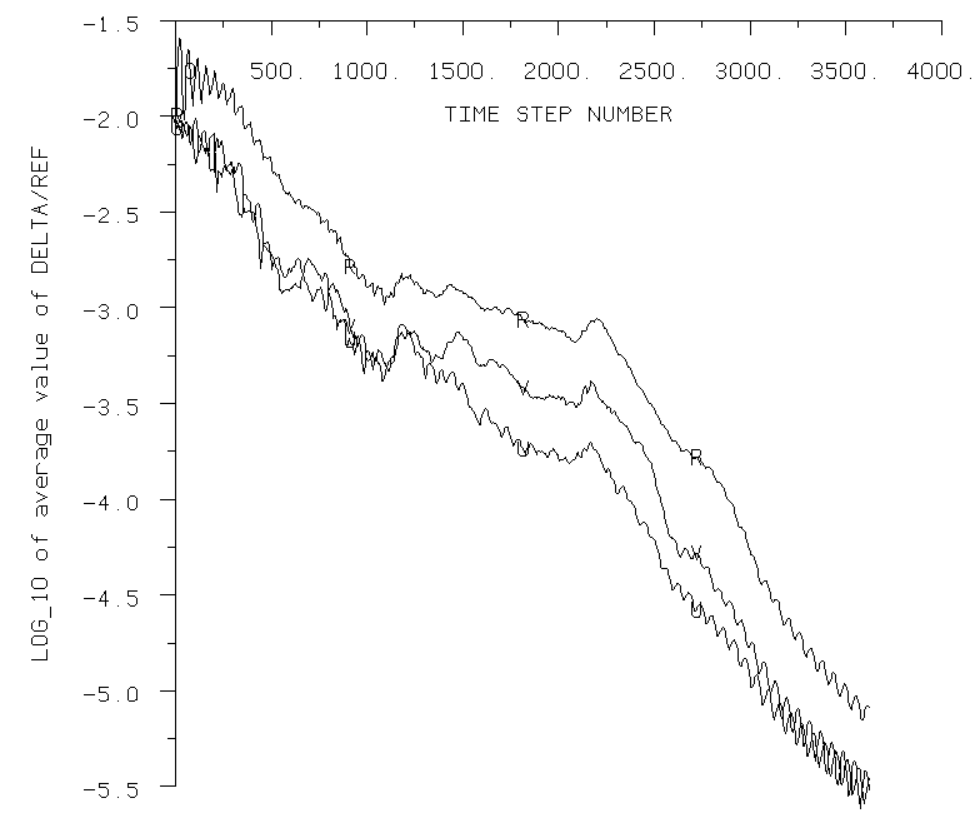
\includegraphics[width=0.7\textwidth]{plots/3.1 conv}
	\caption{Convergence for  best CPU time of test case 3}
	\label{fig:3.1conv}
\end{figure}
\begin{figure}[H]
	\centering
	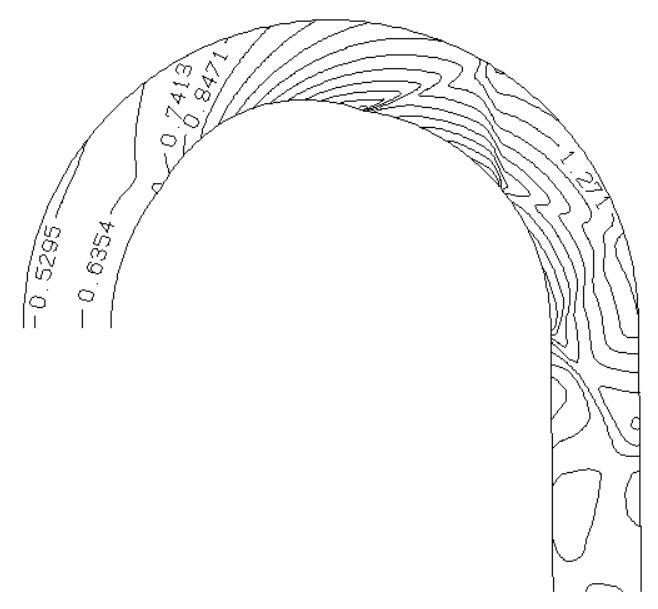
\includegraphics[width=0.7\textwidth]{plots/3.2 mach}
	\caption{Mach contour of test case 3, for $CFL=1.5$ $SF=0.4$}
	\label{fig:3.2mach}
\end{figure}
\autoref{fig:3.1mach}, shows the same oblique shock from test case 2 being formed, but reflecting off the top and bottom surface multiple times. It is difficult to verify the accuracy of this result, however, it can be said the reflections are symmetric (reflected angle = incidence angle). 

Runge-Kutta allowed a much greater $CFL=7.5$ to be used, greater than any other test cases. This led to faster convergence, but the CPU time per step was very low because this geometry contains a large number of nodes and cells. The low $SF=0.05$ allowed the shocks to be captures accurately. \autoref{fig:3.1mach} shows a $SF$ that is just low enough to capture the shocks but also smooth out the unsteadiness on either side of the shocks. \autoref{fig:3.2mach} shows a higher $SF=0.4$, where the shocks have been smeared out with relatively more artificial diffusion. The shocks are still identifiable. Without Deferred Correction, at the same $SF$ the solution would be even more diffused and the shocks would be missed by the CFD as a result.
\subsection{Test Case 4}
This is a wedge of 5.272$\,^{\circ}$ in a fully supersonic flow. A new '\textit{flow\_guess}' and '\textit{apply\_bconds}' were developed to ensure supersonic flow throughout the flow. 
\begin{figure}[H]
	\centering
	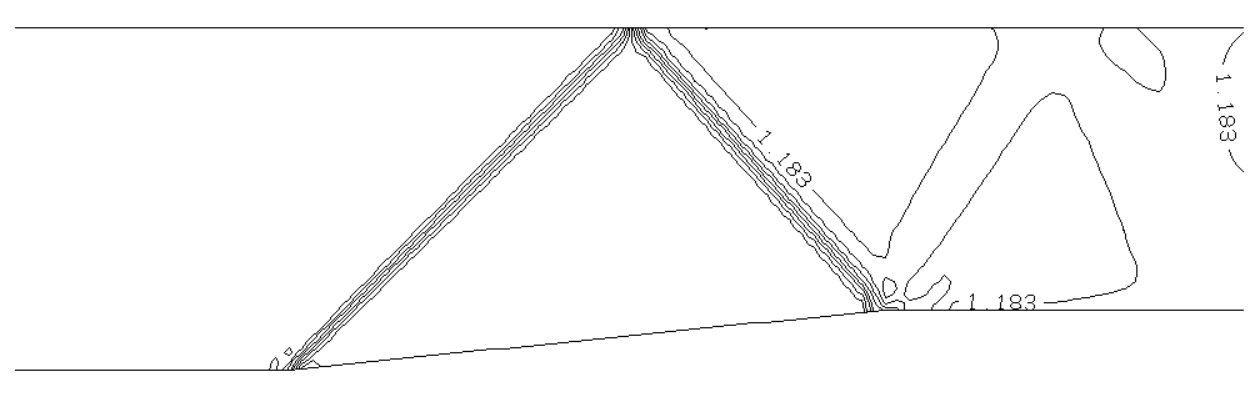
\includegraphics[width=\textwidth]{plots/4.1 mach}
	\caption{Mach contour for  best CPU time of test case 4}
	\label{fig:4.1mach}
\end{figure}
\begin{figure}[H]
	\centering
	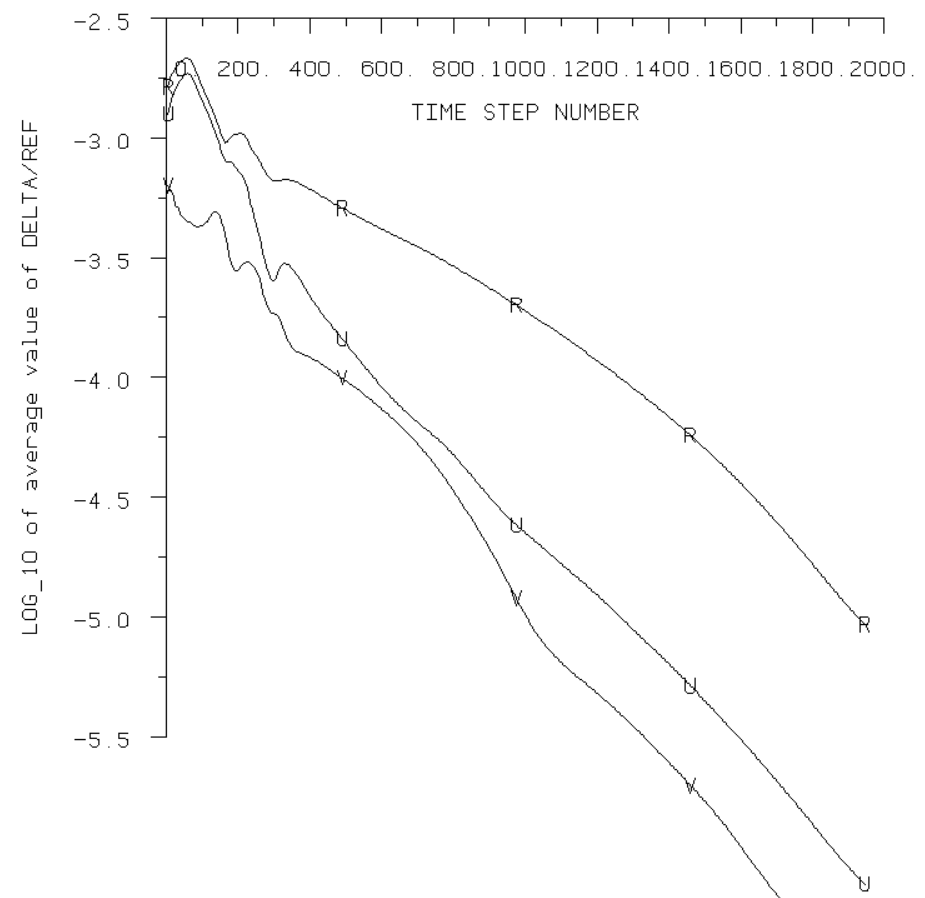
\includegraphics[width=0.7\textwidth]{plots/4.1 conv}
	\caption{Mach contour for  best CPU time of test case 4}
	\label{fig:4.1conv}
\end{figure}
\autoref{fig:4.1mach} shows the distinctive oblique shock wave the the bottom of the wedge, which is reflected to turn the flow back to horizontal. At this $SF$ the solution looks relatively 'clean', with little to no unsteady shock regions shown in the previous cases. Deferred Correction ensures the solution is accurate and not artificially diffused, with the measured outlet Mach being correct to the calculated one to within 0.25\%. Oblique shock tables calculates that the first shock should be at an angle of  44.438$^{\circ}$. From the Mach contour it is measured to be roughly 45$^{\circ}$, again proving how accurate this enhanced code is.

\autoref{fig:4.1conv} shows how smooth the convergence was with little fluctuations in the residuals. This is due to the new flow guess and supersonic boundary conditions which immediately established the supersonic conditions and maintains that.
\begin{figure}[H]
	\centering
	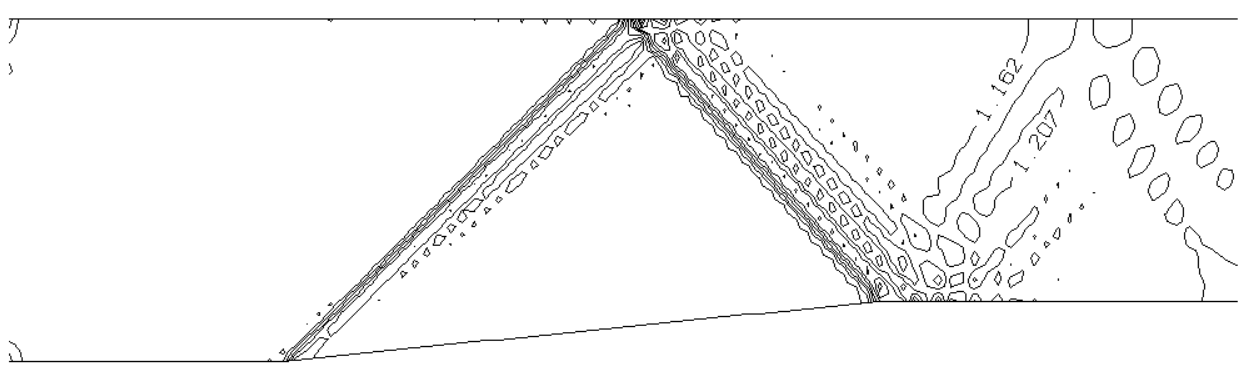
\includegraphics[width=\textwidth]{plots/4.2 mach}
	\caption{Mach contour for minimum $SF$ of test case 4}
	\label{fig:4.2mach}
\end{figure}
At the minimum $SF$ as in \autoref{fig:4.2mach}, some weaker shocks are seen just downstream of the previously identified shocks. This is due to not just a single oblique shocks being formed as one expects from the ideal case. The wedge is not perfectly sharp, as the geometry was defined using discrete numerical points. These weaker shocks result in shocks continue to be reflected as seen from the Mach contour for this lower and hence more accurate $SF$. This observation demonstrates the importance of choosing the $SF$, at a higher $SF$, these weaker shocks were not visualised.
\subsection{Test Case 5}
This is a bend with a sharp corner which has been designed approximately with the method of characteristics to turn a uniform inlet flow at Mach 1 to Mach 3 at the outlet.

\autoref{fig:5.4mach} shows the flow turning and the expansion fan that occurred. The solution is shock free and isentropic as expected. Most importantly, the average Mach at the outlet was measured to be 2.990, which is accurate to the expected 3 to within 0.03\%. This is extremely accurate. Moreover, this test case was expected to produce a uniform flow at outlet which the enclosed contours near the exit suggest. The maximum and minimum Mach at the outlet were measured to be 3.002 and 2.978 respectively. This difference relates to a 0.8\% discrepancy to it being a uniform flow, which is again negligible. \autoref{fig:5.4conv} shows the rapid convergence, with a sudden drop at around step 160. This could be due to the expansion fans being fully developed in the solution and so the iterations suddenly receive little changes.
\begin{figure}[H]
	\centering
	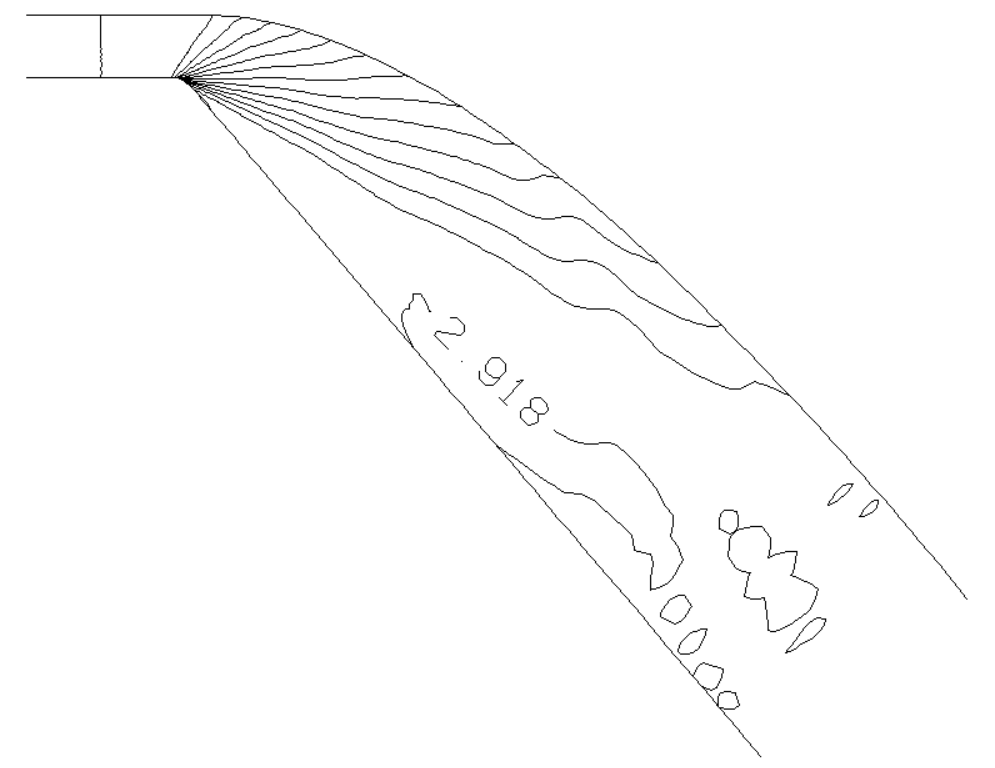
\includegraphics[width=0.75\textwidth]{plots/5.4 mach}
	\caption{Mach contour for  best CPU time of test case 5}
	\label{fig:5.4mach}
\end{figure}
\begin{figure}[H]
	\centering
	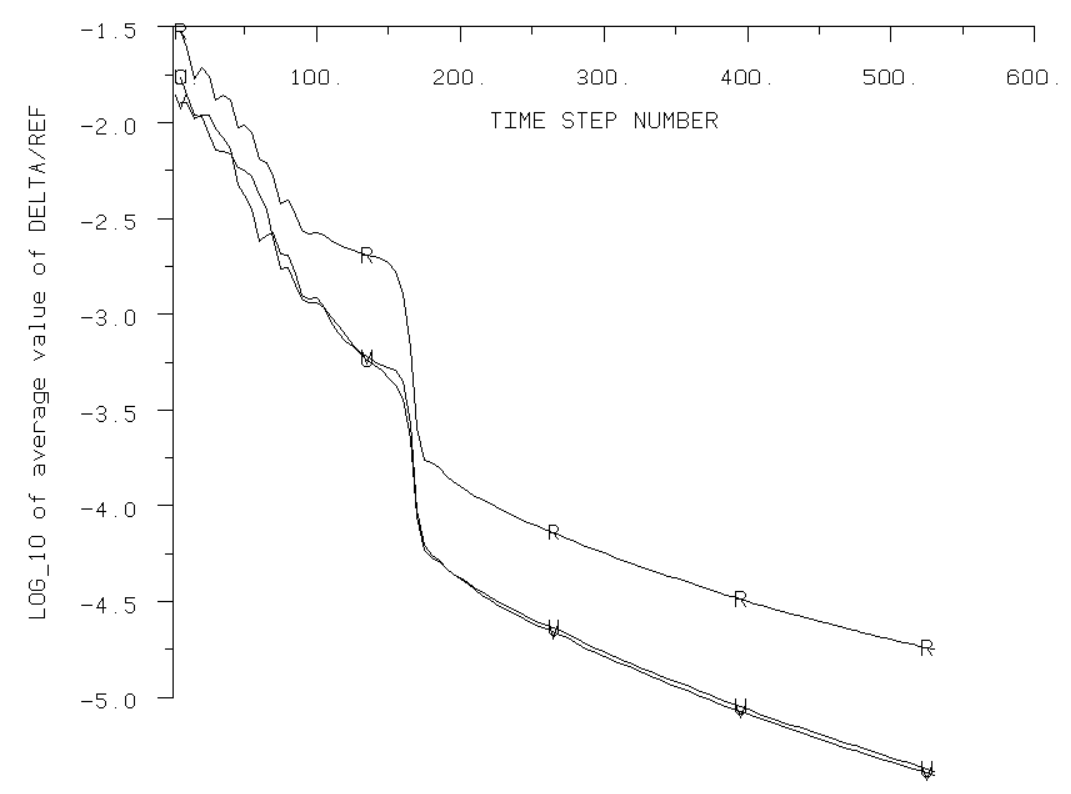
\includegraphics[width=0.7\textwidth]{plots/5.4 conv}
	\caption{Convergence for  best CPU time of test case 5}
	\label{fig:5.4conv}
\end{figure}


\section{Conclusion and Lessons Learned}
CFD is a useful tool to simulate fluid flow behaviour and predict results. However, the basic LAX code initially developed was slow, unstable and inaccurate. The latter was especially important for supersonic flows which relied on accuracy to capture shock waves and their reflections.  4 methods were developed as an extension to the basic code. Runge-Kutta improved stability which allowed larger $CFL$ and $SF$ to be used, at a cost of increased CPU time per step. Deferred Correction increased accuracy by removing artificial viscosity while keeping their stability benefits. Constant stagnation enthalpy and spatially variable time step increased the CPU times.

The results for all 6 test cases show how accurate this enhanced code is, especially supersonic cases which captured the reflected shock waves adequately at an acceptable convergence speed. Although the enhanced code did not improve overall CPU times significantly, the accuracy and stability of the results did, which are equally if not more important in CFD. It also allowed the flexibility in compromising between choosing a lower $SF$ for more accuracy or higher $SF$ for faster convergence. Although in testing it was shown that below $SF=0.25$ the results were still extremely accurate, thanks to Deferred Correction. Lastly, an appropriate $SF$ had to be chosen to not smooth out shock waves which were important when analysing results.


\section{Appendix}\label{sec:Appendix}
\subsection{README}
\small
HOW TO RUN EACH OF THE 6 TEST CASES:

1.  Copy the test case geom and flow into files 'geom' and 'flow'. 
	e.g. for test case 0 in the terminal:
	cp test0\_geom geom
	cp test0\_flow flow

	For other test cases, change above command's 0 to whichever test case number from (0-5)

2.  Edit 'flow' to change CFL and SF as desired. By default they are the best CPU time's CFL and SF. Note for high CFL and/or low SF the solution diverges!

3.  For test cases 4 and 5:
	If geom is copied from the existing test4\_geom or test5\_geom correctly in step 1, by default the correct flow\_guess will be selected in euler.f90. (no need to do anything!)
	Otherwise, check the title in geom is \textbf{"supersonic wedge with M1 = 1.6 "} for test case 4 and \textbf{" Mach 3 Corner "} for test case 5.
	These are checked in euler.f90, lines 56-68. 'flow\_guess\_sup is called' for case 4 and 'new\_guess' for case 5. The variable 'sup' is set to 1 for case 4.

4.  The 4 extensions can be enabled/disabled individually in euler.f90 lines 16-19. Setting = 1 to enable, = 0 to disable. By default all 4 are enabled.

5.  To compile, just run it normally. i.e. in the terminal:
	make clean
	make
	./Euler

\end{document}
